%% MODELO DE LATEX PARA TRABALHOS ACADÊMICOS
%% INSTRUÇÕES GERAIS:
%%    1. TODO O TEXTO NA FRENTE DO SIMBOLO '%' É COMENTÁRIO, ISTO É, ELE NÃO FAZ DIFERENÇA NO RESULTADO FINAL 
%%    2. NESTE MODELO, VOCÊS SÓ PRECISAM EDITAR DAS LINHAS 114 A 132 (INFORMAÇÕES DE CAPA) E DAS LINHAS 188 EM DIANTE (CORPO DO TRABALHO). O RESTO SÃO CONFIGURAÇÕES DE FORMATAÇÃO QUE PROVAVELMENTE NÃO SERÁ PRECISO MODIFICAR.
%%    3. MAIS INSTRUÇÕES DETALHADAS PODERÃO SER ENCONTRADAS NA PÁGINA profhelioh.wordpress.com. DÚVIDAS: heliohenrique@ufpr.br OU heliohenrique3@gmail.com

% INFORMAÇÕES DA FONTE:
%% abtex2-modelo-relatorio-tecnico.tex, v-1.7.1 laurocesar
%% Copyright 2012-2013 by abnTeX2 group at http://abntex2.googlecode.com/ 
%%
%% This work may be distributed and/or modified under the
%% conditions of the LaTeX Project Public License, either version 1.3
%% of this license or (at your option) any later version.
%% The latest version of this license is in
%%   http://www.latex-project.org/lppl.txt
%% and version 1.3 or later is part of all distributions of LaTeX
%% version 2005/12/01 or later.
%%
%% This work has the LPPL maintenance status `maintained'.
%% 
%% The Current Maintainer of this work is the abnTeX2 team, led
%% by Lauro César Araujo. Further information are available on 
%% http://abntex2.googlecode.com/
%%
%% This work consists of the files abntex2-modelo-relatorio-tecnico.tex,
%% abntex2-modelo-include-comandos and abntex2-modelo-references.bib
%%
% ------------------------------------------------------------------------
% ------------------------------------------------------------------------
% abnTeX2: Modelo de Relatório Técnico/Acadêmico em conformidade com 
% ABNT NBR 10719:2011 Informação e documentação - Relatório técnico e/ou
% científico - Apresentação
% ------------------------------------------------------------------------ 
% ------------------------------------------------------------------------

\documentclass[
	% -- opções da classe memoir --
	12pt,				% tamanho da fonte
	% openright,			% capítulos começam em pág ímpar (insere página vazia caso preciso)
    oneside,			% para impressão somente frente. Oposto a twoside (frente e verso)
	a4paper,			% tamanho do papel. 
	% -- opções da classe abntex2 --
	%chapter=TITLE,		% títulos de capítulos convertidos em letras maiúsculas
	%section=TITLE,		% títulos de seções convertidos em letras maiúsculas
	%subsection=TITLE,	% títulos de subseções convertidos em letras maiúsculas
	%subsubsection=TITLE,% títulos de subsubseções convertidos em letras maiúsculas
	% -- opções do pacote babel --
	english,			% idioma adicional para hifenização
	french,				% idioma adicional para hifenização
	spanish,			% idioma adicional para hifenização
	brazil,				% o último idioma é o principal do documento
	]{abntex2}


% ---
% PACOTES
% ---

% ---
% Pacotes fundamentais 
% ---
\usepackage{cmap}				% Mapear caracteres especiais no PDF
\usepackage{lmodern}			% Usa a fonte Latin Modern
\usepackage[T1]{fontenc}		% Selecao de codigos de fonte.
\usepackage[utf8]{inputenc}		% Codificacao do documento (conversão automática dos acentos)
\usepackage{indentfirst}		% Indenta o primeiro parágrafo de cada seção.
\usepackage{color}				% Controle das cores
\usepackage{graphicx}			% Inclusão de gráficos
% ---

% ---
% Pacotes adicionais, usados no anexo do modelo de folha de identificação
% ---
\usepackage{multicol}
\usepackage{multirow}
% ---
	
% ---
% Pacotes adicionais, usados apenas no âmbito do Modelo Canônico do abnteX2
% ---
\usepackage{lipsum}				% para geração de dummy text
% ---

% ---
% Pacotes de citações
% ---
\usepackage[brazilian,hyperpageref]{backref}	 % Paginas com as citações na bibl
\usepackage[alf]{abntex2cite}	% Citações padrão ABNT

% --- 
% CONFIGURAÇÕES DE PACOTES
% --- 

% ---
% Configurações do pacote backref
% Usado sem a opção hyperpageref de backref
\renewcommand{\backrefpagesname}{Citado na(s) página(s):~}
% Texto padrão antes do número das páginas
\renewcommand{\backref}{}
% Define os textos da citação
\renewcommand*{\backrefalt}[4]{
	\ifcase #1 %
		Nenhuma citação no texto.%
	\or
		Citado na página #2.%
	\else
		Citado #1 vezes nas páginas #2.%
	\fi}%
% ---

% ---
% Informações de dados para CAPA e FOLHA DE ROSTO
% ---
\titulo{TESTEMateriais, Métodos e Normas Internacionais para Radioterapia}

\autor{Ana Raquel Santos
	\\
	Daiane Silva
	\\
	Joice Rute
	\\
	Neilane Amaro
	\\
	Rômulo Lima}
\local{Taguatinga}
\data{2016}
\instituicao{%
  Faculdade LS - Lourdes Santana
  \par
  Radiologia}
\tipotrabalho{Relatório técnico}
% O preambulo deve conter o tipo do trabalho, o objetivo, 
% o nome da instituição e a área de concentração 
\preambulo{Trabalho feito para a disciplina Proteção Radiológica no curso de Radiologia.}
% ---

% ---
% Configurações de aparência do PDF final

% alterando o aspecto da cor azul
\definecolor{blue}{RGB}{41,5,195}

% informações do PDF
\makeatletter
\hypersetup{
     	%pagebackref=true,
		pdftitle={\@title}, 
		pdfauthor={\@author},
    	pdfsubject={\imprimirpreambulo},
	    pdfcreator={LaTeX with abnTeX2},
		pdfkeywords={abnt}{latex}{abntex}{abntex2}{relatório técnico}, 
		colorlinks=true,       		% false: boxed links; true: colored links
    	linkcolor=blue,          	% color of internal links
    	citecolor=blue,        		% color of links to bibliography
    	filecolor=magenta,      		% color of file links
		urlcolor=blue,
		bookmarksdepth=4
}
\makeatother
% --- 

% --- 
% Espaçamentos entre linhas e parágrafos 
% --- 

% O tamanho do parágrafo é dado por:
\setlength{\parindent}{1.3cm}

% Controle do espaçamento entre um parágrafo e outro:
\setlength{\parskip}{0.2cm}  % tente também \onelineskip

% ---
% compila o indice
% ---
\makeindex
% ---

% ----
% Início do documento
% ----
\begin{document}

% Retira espaço extra obsoleto entre as frases.
\frenchspacing 

% ----------------------------------------------------------
% ELEMENTOS PRÉ-TEXTUAIS
% ----------------------------------------------------------
% \pretextual

% ---
% Capa
% ---
\imprimircapa
% ---

% ---
% Folha de rosto
% (o * indica que haverá a ficha bibliográfica)
% ---
\imprimirfolhaderosto*
% ---


% ---
% Agradecimentos
% ---
% z
% ---

% ---
% RESUMO
% ---

% resumo na língua vernácula (obrigatório)
% \begin{resumo} %% AQUI COMEÇA A PÁGINA DE RESUMO
%  Segundo a \citeonline{NBR6028:2003}, o resumo deve ressaltar o
%  objetivo, o método, os resultados e as conclusões do documento. A ordem e a extensão
%  destes itens dependem do tipo de resumo (informativo ou indicativo) e do
%  tratamento que cada item recebe no documento original. O resumo deve ser
%  precedido da referência do documento, com exceção do resumo inserido no
%  próprio documento. (\ldots) As palavras-chave devem figurar logo abaixo do
%  resumo, antecedidas da expressão Palavras-chave:, separadas entre si por
%  ponto e finalizadas também por ponto. Bla bla bla bla bla \cite{fulano} %% EXEMPLO DE CITAÇÃO (vá em abntex2-modelo-references.bib)

%  \vspace{\onelineskip}
    
%  \noindent
%  \textbf{Palavras-chaves}: latex. abntex. editoração de texto.
% \end{resumo} %AQUI TERMINA A PÁGINA DE RESUMO
% ---

% ---
% inserir lista de ilustrações
% ---

% \listoffigures* %% o * indica que não será incluso no sumário
\cleardoublepage %% Pula página
% ---

% ---
% inserir lista de tabelas
% ---

% \listoftables*
\cleardoublepage
% ---

% ---
% inserir lista de abreviaturas e siglas
% % ---
% \begin{siglas}
%   \item[Fig.] Area of the $i^{th}$ component
%   \item[456] Isto é um número
%   \item[123] Isto é outro número
%   \item[lauro cesar] este é o meu nome
% \end{siglas}
% ---

% ---
% inserir lista de símbolos
% ---
% \begin{simbolos}
%   \item[$ \Gamma $] Letra grega Gama
%   \item[$ \Lambda $] Lambda
%   \item[$ \zeta $] Letra grega minúscula zeta
%   \item[$ \in $] Pertence
% \end{simbolos}
% ---

% ---
% inserir o sumario
% ---

\tableofcontents*

% ---

% ----------------------------------------------------------
% ELEMENTOS TEXTUAIS  (necessário para incluir número nas páginas)
% ----------------------------------------------------------
\textual


% ----------------------------------------------------------
% Introdução
% ----------------------------------------------------------
\chapter{Objetivo} %% NOVO CAPÍTULO (REPARE QUE ELE AUTOMATICAMENTE JÁ COLOCA O NÚMERO DO CAPÍTULO E JÁ ADICIONA NO SUMÁRIO)

% Aqui você começa a escrever seu trabalho \cite{fulano}. Este documento e seu código-fonte são exemplos de referência de uso da classe
% \textsf{abntex2} e do pacote \textsf{abntex2cite}. O documento 
% exemplifica a elaboração de relatórios técnicos e/ou científicos produzidos
% conforme a ABNT NBR 10719:2011 \textit{Informação e documentação - Relatório
% técnico e/ou científico - Apresentação}.

% \begin{table}[hbt] %% EXEMPLO DE TABELA FEITA POR MEIO DO http://www.tablesgenerator.com/
% \begin{center}
% \caption{Nome da tabela.} %% LEGENDA (REPARE QUE ELE JÁ COLOCA A NUMERAÇÃO AUTOMATICAMENTE E JÁ ADICIONA À LISTA DE TABELAS
% \begin{tabular}{|l|l|lll}
% \cline{1-2}
% Produto & Valor   &  &  &  \\ \cline{1-2}\cline{1-2}
% sdadasd & asdasd  &  &  &  \\ \cline{1-2}
% asdasd  & asasdas &  &  &  \\ \cline{1-2}
% dsad    & asdas   &  &  &  \\ \cline{1-2}
% \end{tabular}
% \end{center}
% \end{table}

% A expressão \textit{\textbf{``Modelo canônico''}} é utilizada para indicar que \abnTeX\ não é
% modelo específico de nenhuma universidade ou instituição, mas que implementa tão
% somente os requisitos das normas da ABNT. Uma lista completa das normas
% observadas pelo \abnTeX\ é apresentada em \citeonline{abntex2classe}. %% USE \citeonline PARA CITAR NO MEIO DA FRASE

% \begin{figure} [hbt] 
% %% hbt SIGNIFICA QUE ELE PRIMEIRO VAI TENTAR COLOCAR A IMAGEM NESTE LUGAR (h de "here"). SENÃO DER, ELE TENTA COLOCAR MAIS PRA BAIXO (b de "bottom"). SENÃO ELE COLOCA MAIS PARA CIMA (t de "top").
% \label{figura1} 
% %% LABEL SERVE PARA VOCÊ REFERENCIAR A FIGURA NO MEIO DO TEXTO (VEJA LINHA 330: \ref{figura1}). ASSIM VOCÊ NÃO PERDE A REFERÊNCIA QUANDO MUDA A FIGURA DE LUGAR
% \caption{Exemplo de figura.}
% % 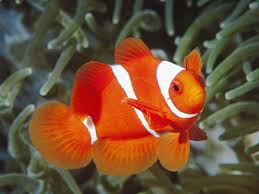
\includegraphics[width=0.95\textwidth]{nemo.jpeg} %% PARA COLOCAR O ARQUIVO DA IMAGEM NO SHARELATEX, CLIQUE NO ÍCONE QUE PARECE UMA FLECHINHA PARA CIMA (ATUALIZAR), CLIQUE EM UPLOAD E PROCURE A IMAGEM EM SEU COMPUTADOR.
% \end{figure}


% Sinta-se convidado a participar do projeto \abnTeX! Acesse o site do projeto em
% \url{http://abntex2.googlecode.com/} (Figura \ref{figura1}). Também fique livre para conhecer,
% estudar, alterar e redistribuir o trabalho do \abnTeX, desde que os arquivos
% modificados tenham seus nomes alterados e que os créditos sejam dados aos
% autores originais, nos termos da ``The \LaTeX\ Project Public
% License''\footnote{\url{http://www.latex-project.org/lppl.txt}}.

% Encorajamos que sejam realizadas customizações específicas deste exemplo para
% universidades e outras instituições --- como capas, folhas de rosto, etc.
% Porém, recomendamos que ao invés de se alterar diretamente os arquivos do
% \abnTeX, distribua-se arquivos com as respectivas customizações.
% Isso permite que futuras versões do \abnTeX~não se tornem automaticamente
% incompatíveis com as customizações promovidas. Consulte
% \citeonline{abntex2-wiki-como-customizar} par mais informações.

% Este documento deve ser utilizado como complemento dos manuais do \abnTeX\ 
% \cite{abntex2classe,abntex2cite,abntex2cite-alf} e da classe \textsf{memoir}
% \cite{memoir}. 

% Equipe \abnTeX 

% Lauro César Araujo


A criação de um Serviço de Radioterapia é um processo longo e abre um grande leque, que envolve muitos recursos financeiros e requer profissionais de diversas áreas. A primeira etapa para criação desse serviço é a escolha e aquisição dos equipamentos que, para os participantes do Programa de Reequipamento Hospitalar do Ministério da Saúde, já foi concluída. A próxima etapa é a criação do Projeto de Blindagem, parte central do Relatório Preliminar de Análise de Segurança (RPAS). Esse documento é um dos que devem ser apresentados à CORAD/CNEN para que o serviço obtenha os registros e autorizações necessárias ao seu funcionamento. Aprovado o RPAS, a CORAD/CNEN emite uma autorização para construção (ou modificação) e o serviço pode iniciar as obras físicas para receber as máquinas. Depois da construção, da instalação dos equipamentos e dos testes de aceitação dos mesmos, deve-se apresentar o Relatório Final de Análise de Segurança (RFAS) - Plano de Radioproteção que, se aprovado, habilitará a operação dos equipamentos e o início do tratamento de pacientes. 

Esse roteiro foi escrito para auxiliar os físicos brasileiros das instituições da ABIFCC, que receberão equipamentos do Ministério da Saúde, na preparação do Relatório Preliminar de Análise de Segurança. O objetivo principal é guiar os profissionais envolvidos nas diferentes etapas, mostrando como se prepara o RPAS de modo que a CORAD/CNEN possa analisa-lo com presteza. O documento deve ser sistematizado com muito cuidado para evitar-se recusa, agilizando a aprovação do projeto e habilitando o serviço a receber os equipamentos. A preparação dessa documentação é de responsabilidade da direção da instituição. O RPAS deve ser elaborado por um profissional experiente, preferencialmente um físico supervisor de radioproteção. Geralmente o grupo encarregado do projeto e construção é composto por: Hospital Contratante, Médico Radioterapeuta, Arquiteto, Físico, Engenheiro Civil, Engenheiro Eletricista, Engenheiro Mecânico, Construtor e Vendedor dos Equipamentos. Para assegurar que o processo transcorra sem problemas é vital que a interação entre esses profissionais seja clara e permanente. A coordenação geral deve ser do arquiteto, com a assistência direta do físico, que trabalharão juntos até o inicio das operações, e que serão o elo entre o contratante e os outros, principalmente entre o fabricante dos equipamentos e o construtor. 

A implementação de um serviço de radioterapia é demorada e o cronograma deve ser realista, incluindo um período adequado para a aceitação dos equipamentos e início dos tratamentos. Além disso, é extremamente importante que todas as exigências legais sejam rigorosamente cumpridas. Dentre elas, destacam-se as autorizações das Secretarias de Saúde e da Coordenação de Instalações Radiativas da CNEN. Nas próximas seções discutiremos em detalhes os itens que devem constar no RPAS. Um prédio para radioterapia não é simplesmente uma construção de tijolos e concreto. Ele envolve também a integração de serviços de energia elétrica, iluminação, condicionamento de ventilação e temperatura, fornecimento de água, drenagem, gases medicinais, acabamento e decoração, tudo conjugado com ergonomia e segurança. Embora os princípios básicos de construção sejam os mesmos, não existe uma solução única do problema e cada caso individual deve ser tratado pela equipe com cuidado e atenção.


% ---
% Capitulo de revisão de literatura
% ---
\chapter{Aspectos Legais}

A portaria 1884/1994 do Ministério da Saúde estabelece que, para a implementação de um serviço de radioterapia onde se possa realizar consultas médicas de programação, preparar o paciente, realizar procedimentos de enfermagem, efetuar o planejamento de tratamento (cálculos, moldes, máscaras, simulação, etc.), aplicar radiações ionizantes terapêuticas com equipamentos apropriados e zelar pela proteção e segurança dos pacientes, operadores e ambiente

Essa mesma portaria determina, ainda, que o serviço deve atender às recomendações da norma CNEN NE-3.06, que trata especificamente da radioproteção e segurança em radioterapia. Este documento estabelece os requisitos necessários para a instalação e operação de um serviço de radioterapia, e suas proposições formam o arcabouço legal que deve ser atendido nos planos de radioproteção. Resumidamente, a norma inicialmente apresenta várias definições, depois apresenta as condições gerais, que incluem a justificação das atividades, as responsabilidades básicas dos diferentes profissionais, as condições de um plano de radioproteção, os requisitos gerais quanto a instalações e equipamentos, os requisitos gerais de radioproteção, os procedimentos e dispositivos de segurança, o controle e monitoração da área, os requisitos de blindagem, os instrumentos de medição necessários, os requisitos de garantia de qualidade, os requisitos de projeto e operação, os registros e inspeções e, finalmente, orientações para o planejamento de instalações e para o projeto das blindagens em radioterapia. Essa apostila segue as recomendações acima, sendo um complemento para seu atendimento.


% --- Seção dentro do capítulo
\section{Papel do Arquiteto}
% ---

Os departamentos de radioterapia devem ser instalados, preferencialmente, em andar térreo, na periferia do complexo hospitalar, para evitar os problemas de radioproteção que surgem se as salas de tratamento estiverem próximas a locais de alta ocupação. Sendo possível, deve ser um bloco independente e exclusivo e sem ocupação sobre o teto. Construções subterrâneas são aceitáveis, mas muito caras, e construções acima do térreo não são recomendadas. A situação em relação ao hospital deve ser tal que facilite a entrada de pacientes ambulatoriais, proporcionando maior facilidade de interação com os outros serviços hospitalares, principalmente a locomoção de pacientes internados e os exames complementares.

A seguir é mostrada uma lista de itens a serem considerados quando se projeta uma sala de tratamento:

Acesso:
\begin{itemize}
	\item Para a máquina;
	\item Para macas e cadeira de rodas;
	\item Segurança;
	\item Blindagem;
	\item Porta de Entrada;
	\item Sinalização de Radiação;
	\item Indicação de FEixe Ligado;
	\item Botões de Emergência;
	\item Microchaves de Segurança;
	\item Comunicação com o Paciente;
	\item Janela ou Circuito Fechado de TV;
	\item Intercomunicação Oral;
	\item Armazenagem Dentro da Sala;
	\item Blocos de blindagem;
	\item Armazenagem na Área de Controle;
	\item Prontuário do Paciente;
	\item Registro dos Tratamentos;
	\item Registro dos Defeitos e Emergências;
	\item Registro de Controle de Qualidade;
	\item Registro do Desempenho da Máquina;
	\item Equipamentos de Dosimetria;
	\item Equipamentos de Testes;
	\item Peças de Reposição;
	\item Dispositivos de Alinhamento por Laser;
	\item Controle de Iluminação;
	\item Energia Elétrica;
	\item Para a Máquina;
	\item Para os Instrumentos de Dosimetria;
	\item Água e Esgoto;
	\item Gases Medicinais;
	\item Decoração;
	\item Acomodação dos Pacientes;
	\item Sala de Espera;
	\item Sala de Troca de Roupa;

\end{itemize}
	
Esses são alguns dos exemplos de uma sala de radioterapia, quando se projetada.

\section{Papel do Engenheiro}

O papel dos engenheiros é assegurar que a sala do equipamento possa ser construída da maneira como foi planejada. Para paredes de concreto isso inclui a armação e a concretagem e, se forem usadas placas de aço ou chumbo, a forma como elas serão fixadas nos locais apropriados. Deve-se assegurar que o método de construção é tal que não existirão buracos ou juntas pelas quais a radiação possa escapar, e, que as especificações e os controles dos materiais, dosagem (composição), densidade, propriedades mecânicas, elásticas e térmicas são as necessárias e atendem ao projeto.

O acabamento e a decoração compõem a parte final do projeto. Ela deve ser planejada cuidadosamente, se possível com a assistência de arquiteto de interiores. A primeira preocupação deve ser a da facilidade de limpeza e desinfecção. Paredes pintadas a óleo, piso de granito e teto rebaixado de gesso oferecem acabamento adequado. As cores, texturas, mobiliário, etc., devem ser tais que proporcionem sensação de tranquilidade e limpeza.

\chapter{Detalhamento}

O acesso às salas de tratamento deve ser largo o suficiente para tornar possível a entrada da máquina, de macas e cadeiras de rodas. O piso deve suportar o peso dos equipamentos e permitir que as caixas circulem sem interferências. Uma sala com labirinto bem projetado, pode não exigir blindagem na entrada, a existência de uma barreira física é imprescindível para evitar a circulação de pessoas não autorizadas. A blindagem da porta é necessária quando não se tiver espaço suficiente para um bom labirinto ou quando a sala receber novo equipamento de energia mais alta. Portas motorizadas devem ter um mecanismo auxiliar que permita a sua abertura no caso de falha mecânica ou elétrica. 

É imprescindível que a porta possa ser aberta de ambos os lados e, embora não exija fechadura, deve-se instalar um dispositivo, por exemplo, magnético, que assegure o fechamento numa exposição. A blindagem da porta deve ser contínua e homogênea e se estender alguns centímetros além do vão de entrada para evitar a existência de frestas. A sala de controle deve se situar próxima à porta para que os técnicos mantenham vigilância permanente no acesso e para que seu trabalho seja realizado com mais eficiência e presteza. É importante a instalação de uma chave geral para desligar tudo numa emergência. Para evitar danos aos equipamentos, todas as tomadas devem ser aterradas e estar ao mesmo potencial e fase. Deve-se afixar na porta o sinal internacional de presença de radiação (trifólio) com dizeres CUIDADOS – RADIAÇÃO e telefones dos responsáveis e de quem acionar em casos de emergência. Um sinal automático de aviso de prontidão para irradiar e outro de presença de radiação deve-se fazer presente e visível na mesa de controle, na entrada sobre a porta e dentro da sala de tratamento. 

 Para equipamentos de telecobalterapia ou de braquiterapia de alta taxa de dose, deve-se instalar um detector ambiental de radiação independente (GM ou similar), com sinalização de exposição na mesa de controle e na entrada da sala. Botões de emergência devem ser instalados nas áreas de controle e de tratamento. As salas de tratamento exigem a instalação de sistema de água para resfriamento do acelerador linear, de água e esgoto para higiene das mãos e para dosimetria. É necessário um sistema de ar condicionado e, muitas vezes, de um sistema de gases medicinais para anestesia e recuperação do paciente. 

 A entrada de todos os tubos na sala deve ficar fora do feixe primário e devem ser curvos, de modo a evitar o escape de radiação, piso e recessos devem ser impermeabilizados. A drenagem do solo é um dos primeiros itens na construção, e deve ser executada com técnica apurada. O sistema de ar condicionado deve climatizar adequadamente o ambiente e proporcionar recirculação do ar. O duto de entrada deve ser blindado por lâminas de chumbo ou por absorvedores de foto nêutrons.  Várias tomadas e interruptores elétricos devem ser instalados nas paredes da sala, principalmente próximas ao gantry. Elas são necessárias para a iluminação, para os lasers de posicionamento, para serviços de limpeza e manutenção, para os equipamentos de dosimetria, para as câmaras de TV, para o monitor ambiental de radiação, para ventiladores, quando o sistema de ar condicionado entra em pane, para os botões de emergência, para os sinalizadores, etc. 

 Para assegurar a radioproteção adequada, caso as caixas de passagem ou lasers sejam embutidos nas paredes blindadas, deve-se fixa-los em placas de aço fundidas no concreto com dimensões de 4 cm de espessura e margem extra de 2,5 cm em relação à caixa. 

 A visualização do paciente é mandatária e idealmente deve ser feita com duas câmaras de TV, posicionadas defronte ao aparelho para ótima monitoração, Nenhum tratamento pode ser realizado se o paciente não for visualmente monitorado. A instalação de um sistema de intercomunicação oral de duas vias é mandatária e deve ser feito entre a sala de controle e a de tratamento, permitindo que tanto a voz do técnico quanto à do paciente sejam audíveis. 

Recomenda-se a instalação de piso antiestático nas salas de tratamento e controle, já que vários computadores, dispositivos eletrônicos e gases inflamáveis serão usados. Um item extremamente importante e muitas vezes negligenciado é a instalação de duto apropriado para passagem de cabos de dosimetria. Devemos nos lembrar de que a dosimetria moderna exige uma variedade de cabos como, pôr exemplo, para calibração padrão, para movimentação automática de câmaras de ionização dentro de fantomas, para dosimetria in-vivo, para conexão de computadores, etc. 

 A presença de lintel interno, que muitas vezes é exigida pela estrutura, é uma boa forma de reduzir a radiação espalhada no labirinto, principalmente para foto nêutrons. 


\chapter{Estrutura geral do RPAS}

O Relatório Preliminar de Análise de Segurança (RPAS) é o documento necessário para conseguir a autorização de construção e importação dos equipamentos geradores de radiação ionizante junto a CNEN. Mas para estar aptos a operar os equipamentos é necessário obter-se junto a CNEN, a licença de operação. 

É necessário que haja junto ao documento, uma solicitação de Concessão de Licenças autorizadas (SCRA), obrigatório. Desde 1999 a CNEN foi autorizada a cobrar taxas de licenciamento. 

O RPAS deve conter claras informações, como transporte de rejeitos quando aplicáveis, definição de sigla, símbolos, termos especiais (etc.) 

O RPAS deve conter as seguintes especificações: Somente em Papel A4, esquemas e gráficos dobrados em tamanho A4, plantas em alta escala com o carimbo de identificação na frente com assinatura e número de registro na CNEN do supervisor de radioproteção e a assinatura do diretor responsável pela instituição. Devem conter ao menos três plantas, uma localizando o serviço de radioterapia e o hospital em relação a vizinhança, a outra planta do serviço de radioterapia identificando todas as instalações e sua vizinhança, e a terceira planta contendo detalhes da área blindada. 

É necessário conter toda a identificação da empresa. Colocar todas as informações para a identificação completa de todos os equipamentos emissores de radiação ionizante, com detalhes de sua situação. Descrever o funcionamento do equipamento com anexos de catálogos. Apresentar todos os trabalhadores e suas qualificações. Identificar os monitores portáteis de área e o dosímetros clínicos. Descrever detalhadamente as instalações \cite{talbot2012}.



% ---
% Conclusão
% ---


% ----------------------------------------------------------
% ELEMENTOS PÓS-TEXTUAIS
% ----------------------------------------------------------
\postextual


% ----------------------------------------------------------
% Referências bibliográficas
% ----------------------------------------------------------
% \bibliographystyle{abbrv}
\bibliography{abntex2-modelo-references} %% REFERENCIA AO ARQUIVO abntex2-modelo-references.bib

% ----------------------------------------------------------
% Glossário
% ----------------------------------------------------------
%
% Consulte o manual da classe abntex2 para orientações sobre o glossário.
%
%\glossary

% ----------------------------------------------------------
% Apêndices
% ----------------------------------------------------------

% ---
% Inicia os apêndices
% ---
% \begin{apendicesenv}

% % Imprime uma página indicando o início dos apêndices
% \partapendices

% % ----------------------------------------------------------
% \chapter{Quisque libero justo}
% % ----------------------------------------------------------

% \lipsum[50]

% % ----------------------------------------------------------
% \chapter{Nullam elementum urna vel imperdiet sodales elit ipsum pharetra ligula
% ac pretium ante justo a nulla curabitur tristique arcu eu metus}
% % ----------------------------------------------------------
% \lipsum[55-57]

% \end{apendicesenv}
% ---


% ----------------------------------------------------------
% Anexos
% ----------------------------------------------------------

% ---
% Inicia os anexos
% ---
% \begin{anexosenv}

% % Imprime uma página indicando o início dos anexos
% \partanexos

% % ---
% \chapter{Morbi ultrices rutrum lorem.}
% % ---
% \lipsum[30]

% % ---
% \chapter{Cras non urna sed feugiat cum sociis natoque penatibus et magnis dis
% parturient montes nascetur ridiculus mus}
% % ---

% \lipsum[31]

% % ---
% \chapter{Fusce facilisis lacinia dui}
% % ---

% \lipsum[32]

% \end{anexosenv}

%---------------------------------------------------------------------
% INDICE REMISSIVO
%---------------------------------------------------------------------

\printindex

% http://www.cnen.gov.br/requerimentos-referente-a-licenciamentos
% http://www.oncoguia.org.br/conteudo/equipe-multidisciplinar/4618/698/

%---------------------------------------------------------------------
% Formulário de Identificação (opcional)
%---------------------------------------------------------------------
% \chapter*[Formulário de Identificação]{Formulário de Identificação}
% \addcontentsline{toc}{chapter}{Exemplo de Formulário de Identificação}
% \label{formulado-identificacao}

% Exemplo de Formulário de Identificação, compatível com o Anexo A (informativo)
% da ABNT NBR 10719:2011. Este formulário não é um anexo. Conforme definido na
% norma, ele é o último elemento pós-textual e opcional do relatório.

% \bigskip

% \begin{tabular}{|p{9cm}|p{5cm}|} %% EXEMPLO DE TABELA MAIS COMPLEXA
% \hline
% \multicolumn{2}{|c|}{\textbf{\large Dados do Relatório Técnico e/ou científico}}\\
% \hline
% \multirow{4}{10cm}[24pt]{Título e subtítulo}& Classificação de segurança\\
%                    & \\
%                    \cline{2-2}
%                    & No.\\
%                    & \\
				
% \hline
% Tipo de relatório & Data\\
% \hline
% Título do projeto/programa/plano & No.\\
% \hline
% \multicolumn{2}{|l|}{Autor(es)} \\
% \hline
% \multicolumn{2}{|l|}{Instituição executora e endereço completo} \\
% \hline
% \multicolumn{2}{|l|}{Instituição patrocinadora e endereço completo} \\
% \hline
% \multicolumn{2}{|l|}{Resumo}\\[3cm]
% \hline
% \multicolumn{2}{|l|}{Palavras-chave/descritores}\\
% \hline
% \multicolumn{2}{|l|}{
% Edição \hfill No. de páginas \hfill No. do volume \hfill Nº de classificação \phantom{XXXX}} \\
% \hline
% \multicolumn{2}{|l|}{
% ISSN \hfill \hfill Tiragem \hfill Preço \phantom{XXXXXXXX}} \\
% \hline
% \multicolumn{2}{|l|}{Distribuidor} \\
% \hline
% \multicolumn{2}{|l|}{Observações/notas}\\[3cm]
% \hline
% \end{tabular}

\end{document}
